\documentclass[12pt,a4paper]{paper}
    \usepackage[utf8]{inputenc}
    \usepackage{amsmath}
    \usepackage{amsfonts}
    \usepackage{amssymb}
    \usepackage[danish]{babel}
    \usepackage{graphicx}
    \usepackage{natbib}
    \usepackage{siunitx}
    \usepackage{fancyhdr}
    %Graf usepackage
    \usepackage{tikz}
    \usepackage{pgfplots}
    \usepackage{tkz-euclide}
    % Start på divi peamble
    \usepackage{xcolor}
    \usepackage{multirow}
    \usepackage{booktabs}
    \usepackage{xparse}
    \usepackage{calc}

    
    \author{Gruppe 16}
    \title{CDIO3}
    \pagestyle{fancy}
    \lhead{Gruppe 16}
    \rhead{CDIO3}
    \chead{1. december 2017}

% Hejsa,
% Opret et underdokument til hver underogpave (Anlyse / Design / Implementering / osv)
% GO - Btw, er i ikke primus på en opgave, så ændrer for Guds skyld ikke i den. Hold jer til jeres eget shit ;-)
    \begin{document}
        \section{Analyse}
        
    
    \subsection{Kravliste}
        \begin{enumerate}
<<<<<<< HEAD
<<<<<<< HEAD
<<<<<<< HEAD
            \item Spillet skal være mellem 2 - 4 personer
            \item Spillerne skal slå terninger på skift
            \item Der skal udskrives en tekst der omhandler det aktuelle felt, når spilleren lander på et felt
            \item Hver felt skal have en effekt for spilleren
            \item Spillerne starter med en balance på:
            \begin{enumerate}
                \item 20, hvis der er 4 spillere.
                \item 18, hvis der er 3 spillere.
                \item 16, hvis der er 2 spillere.
            \end{enumerate}
            %Efter de nye regler så starter spillerne med hhv. 20, 18 eller 16 Matadollars, alt efter om der er 2, 3 eller 4 spillere.
            \item Spillet slutter når den første spiller har mistet alle sine penge.
            %Efter de nye regler så er der når den første spille går bankerot
            \item Spillerne skal kunne gå flere omgange rundt på spillepladen.
            \item Spillet skal kunne køre på DTU’s databarer.
        \end{enumerate}

%---------------------------------------------------------------------------
%                             Input af usecases
%--------------------------------------------------------------------------
\input{UseCases.tex}

<<<<<<< HEAD
\subsection{UseCases}
%1. UseCase
\begin{center}
\begin{tabular}{ | m{10em} | m{10cm}| }
        \hline
            UseCase Section: Opsætning af spil & Comment\\
        \hline
            Scope & Monopoly spil af IOOuterActive\\
        \hline
            Level & User-goal\\
        \hline
            Primær Aktør & Spillerne\\
        \hline
            Stakeholder og interessenter & Spillerne er interesserede i at kunne starte spillet ved at vælge antal spillere og deres brikker\\
        \hline
            Forudsætninger & Spillet bliver kørt, og spillerne har nu mulighed for at vælge antal spillere og ønskede brikker\\
        \hline
            Success guaranti & Der er blevet valgt antallet af spillere, og hver spiller har valgt sin brik, herefter er spillet klar til at blive spillet\\
        \hline
    \end{tabular}
\end{center}
%2. UseCase
\pagebreak
Fully dressed UseCase:
\begin{center}
\begin{tabular}{ | m{10em} | m{10cm}| }
        \hline
            UseCase Section: Spillerne slår med terningerne & Comment\\
        \hline
            Scope & Monopoly spil af IOOuterActive\\
        \hline
            Level & User-goal\\
        \hline
            Primær Aktør & Spillerne\\
        \hline
            Stakeholder og interessenter & Spillerne er interesseret i at kunne trykke på en knap, og få et billede af to terninger med tilfældige værdier\\
        \hline
            Forudsætninger & Spillet er startet op, og spillerne har valgt antallet spillere og deres ønskede brikker\\
        \hline
            Success guaranti & Der er blevet valgt antallet af spillere, og hver spiller har valgt sit navn, herefter er spillet klar til at blive spillet\\
        \hline
            Hoved succes scenarie & Spillerne får udgivet en værdi af to terninger, og lander derefter på et felt\\
        \hline
            Alternative udfald & Negative udfald:\\
                & -	IOOuterActive har opdateret spillet, og derved opstår der en fejl når spillerne slå med terningerne, der kan ende i at der ikke bliver slået to terninger\\
                & -	Systemet blokerer for en spillers tur\\
                & -	En spiller hopper fra/på, og derved skal spillet startes om\\
        \hline
            Specielle krav
            & -	Enheden som spillet kører på skal være kompatibel med Java\\
            & -	Spillerne skal kunne interagere med GUI’en ved brug af mus eller touch\\
            & -	Der skal være plads på enheden til at kunne hente spillet\\
        \hline
            Hyppighed & Hver tur bliver der slået med terninger\\
        \hline
    \end{tabular}
\end{center}

%3. UseCase
\begin{center}
\begin{tabular}{ | m{10em} | m{10cm}| }
        \hline
            UseCase Section: Spiller lander på et felt & Comment\\
        \hline
            Scope & Monopoly spil af IOOuterActive\\
        \hline
            Level & User-goal\\
        \hline
            Primær Aktør & Spillerne\\
        \hline
            Stakeholder og interessenter & Spillerne er interesseret hvilken effekt de kommer i møde når de lander på et felt\\
            Hvis feltet ikke er opkøbt af nogen, kan spilleren der er landet på feltet købe det, medmindre det er et specielt felt\\
            Hvis feltet er ejet af nogen, skal spilleren der er landet på feltet betale den der ejer feltet\\
            Feltet de lander på kan også være et fængsel, der gør at spilleren mister en tur 
        \hline
            Forudsætninger & Spillet er i gang og en spiller har slået med terningerne\\
        \hline
            Success guaranti & Spilleren køber og ejer nu feltet\\
        \hline
    \end{tabular}
\end{center}

%4. UseCase
\begin{center}
\begin{tabular}{ | m{10em} | m{10cm}| }
        \hline
            UseCase Section: Spiller trækker et chancekort & Comment\\
        \hline
            Scope & Monopoly spil af IOOuterActive\\
        \hline
            Level & User-goal\\
        \hline
            Primær Aktør & Spillerne\\
        \hline
            Stakeholder og interessenter & Spillerne er interesseret i hvilken bonus de får når de trækker et chancekort\\
        \hline
            Forudsætninger & Spillet er i gang og en spiller trækker et chancekort\\
        \hline
            Success guaranti & En spiller lander trækker et chancekort og får en belønning eller en straf\\
        \hline
    \end{tabular}
\end{center}

%5. UseCase
\begin{center}
\begin{tabular}{ | m{10em} | m{10cm}| }
        \hline
            UseCase Section: Spillet afsluttes & Comment\\
        \hline
            Scope & Monopoly spil af IOOuterActive\\
        \hline
            Level & User-goal\\
        \hline
            Primær Aktør & IOOuterActive\\
        \hline
            Stakeholder og interessenter & IOOuterActive er interesserede i at programmet viser en vinder og afsluttes\\
        \hline
            Forudsætninger & Alle spillere undtagen en, har fået en balance på 0\\
        \hline
            Success guaranti &Spillet viser en vinder og kan derefter afsluttes\\
        \hline
    \end{tabular}
\end{center}
\subsection{UseCase-Diagram}
\includegraphics[scale=0.8]{fig/dtu/UC-cdio3.jpg}
=======
=======
            \item Spillet skal være mellem 2 - 4 personer.
            \item Spillerne skal slå med en terningen på skift.
            \item Der skal udskrives en tekst, der omhandler det aktuelle felt, når spilleren lander på et felt.
            \item Spilleren skal købe feltet, hvis der landes på et frit felt.
            \item Spilleren skal betale husleje til ejeren, hvis der landes på et købt felt.
            \item Spilleren skal betale dobbelthusleje til ejeren, hvis der landes på en "par"-ejet hustand.
            \item Spillere modtager 2M, når start passeres.
            \item Spilleren ryger direkte i fængsel, hvis der landes på "GÅ I FÆNGSEL". Der modtages ikke 2M, hvis start passeres i forbindelse med dette.
            \item Sidder man i fængsel, bliver ens "Du løslades uden omkostninger"-kort brugt. Hvis kortet ikke haves betales der 1M.
            \item Landes der på "Chance", bliver effekten printet, og den printede effekt sker.
            \item Landes der på "Gratis parkering" sker ingenting, og turen går videre.
            \item Landes der på "På besøg" sker ingenting, og turen går videre.

            \item Spillerne starter med en balance på:
            \begin{enumerate}
                \item 16, hvis der er 4 spillere.
                \item 18, hvis der er 3 spillere.
                \item 20, hvis der er 2 spillere.
            \end{enumerate}
            %Efter de nye regler så starter spillerne med hhv. 20, 18 eller 16 Matadollars, alt efter om der er 2, 3 eller 4 spillere.
            \item Spillet slutter, når den første spiller har mistet alle sine penge.
            \item Spilleren med flest penge vinder, når spillet slutter vinder. Efterfølgende printes "Tillykke (spiller)", du har vundet!"

            %Efter de nye regler så er der når den første spille går bankerot
            \item Spillerne skal kunne gå flere omgange rundt på spillepladen.
            \item Spillet skal kunne køre på DTU’s databarer.

        \end{enumerate}

=======
            \item Spillet skal være mellem 2 - 4 personer.
            \item Spillerne skal slå med en terningen på skift.
            \item Der skal udskrives en tekst, der omhandler det aktuelle felt, når spilleren lander på et felt.
=======
            \item Spillet skal være mellem 2 - 4 personer
            \item Spillerne skal slå terninger på skift
            \item Der skal udskrives en tekst der omhandler det aktuelle felt, når spilleren lander på et felt
>>>>>>> parent of 80653f5... +Rettelser i rapport
            \item Spilleren skal købe feltet, hvis der landes på et frit felt.
            \item Spilleren skal betale husleje til ejer, hvis der landes på et købt felt
            \item Spilleren skal betale dobbelthusleje til ejer, hvis der landes på et "par".
            \item Spillere modtager 2M, når start passeres.
            \item spilleren ryger direkte i fængsel, hvis der landes på "GÅ I FÆNGSEL". Der modtages ikke 2M, når start passeres.
            \item Sidder man i fængsel, bliver ens "Du løslades uden omkostninger"-kort brugt. Hvis kortet ikke haves betales der 1M.
            \item Landes der på "Chance", bliver effekten printet og den printede effekt sker.
            \item Landes der på "Gratis parkering" sker ingenting, og turen går videre.
            \item Landes der på "På besøg" sker ingenting, og turen går videre.

            \item Spillerne starter med en balance på:
            \begin{enumerate}
                \item 16, hvis der er 4 spillere.
                \item 18, hvis der er 3 spillere.
                \item 20, hvis der er 2 spillere.
            \end{enumerate}
            %Efter de nye regler så starter spillerne med hhv. 20, 18 eller 16 Matadollars, alt efter om der er 2, 3 eller 4 spillere.
            \item Spillet slutter når den første spiller har mistet alle sine penge.
            \item Spilleren med flest penge vinder, når spillet slutter, og der printes "Tillykke "vinder", du har vundet!"

            %Efter de nye regler så er der når den første spille går bankerot
            \item Spillerne skal kunne gå flere omgange rundt på spillepladen.
            \item Spillet skal kunne køre på DTU’s databarer.

        \end{enumerate}

>>>>>>> 80653f595c5290349d98a062999656c5144bf36c
%---------------------------------------------------------------------------
%                             Input af usecases
%--------------------------------------------------------------------------
\input{UseCases.tex}

<<<<<<< HEAD
>>>>>>> 80653f595c5290349d98a062999656c5144bf36c
=======
>>>>>>> 80653f595c5290349d98a062999656c5144bf36c
\pagebreak
\subsection{UseCase diagram}
    \begin{figure}[h]
        \advance\leftskip-3cm
        \includegraphics[width=20cm]{fig/UC-cdio3.jpg}
        \caption{UseCase diagram tegnet i MagicDraw}
    \end{figure}
<<<<<<< HEAD
<<<<<<< HEAD
>>>>>>> e63a5fd0f6c23ba43f52a4b27a512b9be4955e76
=======
>>>>>>> 80653f595c5290349d98a062999656c5144bf36c
=======
>>>>>>> 80653f595c5290349d98a062999656c5144bf36c

\subsection{GRASP}
    GRASP står for \textit{General Responsibility Assignment Software Patterns}. GRASP bruges til at give det rigtige ansvar til de forskellige klasser, der bliver oprettet under udviklingen af et program. GRASP indeholder 9 patterns. Patterns bliver brugt til at strukturere et problem, samt at finde en passende løsning. De 9 patterns er:
        \begin{enumerate}
            \item Creator
            \item Information expert
            \item Low coupling
            \item Controller
            \item High cohesion
            \item Indirection
            \item Polymorphism
            \item Protected variations
            \item Pure fabrication
        \end{enumerate}
    (Der skrives mere når vi er nået længere i projektet)

        \pagebreak
        \section{Design}

\subsection{Klasse diagram}
    Udkast af klasse diagram lavet og det ligger nu i drive og på GitHub. 
    Nogen spørgsmål spørg endelig.
    

\subsection{Sekvensdiagram}
    Udkast af sekvens diagram lavet og det ligger nu i drive og på GitHub. 
    Nogen spørgsmål spørg endelig.

\subsection{Domænemodel}
        \pagebreak
        %%\input{test.tex}
    \end{document}